\documentclass[12pt]{article}

\usepackage{tabularx}
\usepackage{pdflscape}
\usepackage{float}
\usepackage{graphicx}

\newcommand{\mypath}{./figures/}
\graphicspath{\mypath}


\title{World Robotic Sailing Championship 2018 \\
Notice of race and competition rules \\v1.1}
\date{\today}

\begin{document}
\maketitle
% GOALS:
% - Scoring based on data, measurable success
% - KISS -> simplify as far as possible
% - Additive success: No loss of all points, generally no loss of points!
% - clear and unambiguous: Don't assume things are implied, avoid formulations
%   that may lead to rule discussions.

\section{Introduction}

The World Robotic Sailing Championship 2018 will be organized in Southampton,
UK, from 26\textsuperscript{th} to 30\textsuperscript{th} of August.
The World Robotic Sailing Championship will be followed by
the International Robotic Sailing Conference that will be held on August
31\textsuperscript{st} and September 1\textsuperscript{st} at the University of
Southampton.
The organizing committee invites teams from any organization, including private
individuals, schools, colleges, universities and companies, to enter the competition. 
Each team competes with one boat; the team members can be shared among different teams. 
The championship will be organized in 4 challenges, each one tentatively allocated to a single day.

\section{Classes}

The World Robotic Sailing Championship is open to all vessels using 
only wind and wave energy for propulsion. 
Besides the more traditional soft or rigid sailing rigs, wind energy may also 
be used to power a propeller or a paddle-wheel driven by a wind turbine. 
The coupling between the wind turbine and the propulsion unit may be done by 
mechanical or electrical means, providing that the use of other energy sources
is clearly inhibited. The teams must be able to clearly demonstrate 
this to the race committee.
Vessels may use any type of hull (mono or multi) and any type of rig, with
one or more soft or rigid sails. The beam of multi-hulls should not exceed their 
LOA (length overall, maximum length of the hull measured parallel to the waterline) 
and the maximum draft of any boat should be limited to 2 m. 
Hydrofoils are allowed. Sails and appendages may be changed between challenges.

The two classes considered in WRSC 2018 are:
\begin{itemize}
  \item Micro-sailboats (MS): small autonomous sailboats up to 1.5 m LOA and weighting no more than 100 kg.
  \item Sailboats (S): autonomous sailboats which do not fit in the micro-sailboats category, up to
4.2 meters LOA and weighting no more than 500 kg.
\end{itemize}

\section{Liability and Safety}
All sailing robots must be controllable by a designated human helmsman
throughout all events. The responsibility for avoiding any collision, 
damage or personal injuries will rest solely with the respective teams. 
The organizers will not assume any liability with respect to third party
damages, personal injuries or environmental contamination resulting from any
activity of a team participating in the WRSC. All teams are responsible for 
their own safety during the event and the decision to participate in the 
competitions is of the exclusive responsibility of the team members.
Before being allowed to compete, each team has to register a person of contact
who will be held responsible for any damage, injury or environmental
contamination resulting from any activity of the team, including the 
operation of their vessel.

All sailing boats will be under the supervision of support vessels provided by the
organization.
All people on board of a support vessel must follow the safety instructions of the driver 
and must provide their own personal floatation device which must be worn at all times 
while on or near the water. We aim to allow at least one member per team on a support vessel, 
however the organisers reserve the
right to manage the fleet of support vessels, and can refuse access to the support
vessels for any reason.
All team members must follow the instructions of the competition
organisers, the support vessel crew, and the activity centre personnel. The organizers
reserve the right to refuse access to restricted areas.
For safety reasons, the race area may be confined to a region delimited by 4
marks. 


  \begin{figure}[H]
    \centering
    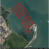
\includegraphics[width=0.6\textwidth]{competition-area}
    \caption{The approximate race area reserved for WRSC}
    \label{fig:competitionarea}
  \end{figure}

  Figure \ref{fig:competitionarea} shows approximately the area requested for WRSC that may be subject to last
minute adjustments.


\section{Collisions and Right of Way}
Autonomous boats have right of way over manually controlled boats. In the event
of a potential
collision, then COLREGs rules must be followed (for example, a boat on a
starboard tack has
right of way, etc). However, all competitors must take appropriate actions to
avoid collisions
and having right of way is not an acceptable excuse for allowing a collision to
take place.
Remote control is allowed to avoid imminent collisions for the boat with no 
right of way. Alternatively, a collision may also be
prevented by manually holding the boat with no right of way, but ensuring that 
its position and heading is maintained until the risk of collision has passed. 
In the case a boat gets entangled with a buoy or any other
floating debris (seaweed, lines, fishing nets, etc) it can be assisted manually,
as long as no advantage is given to the boat and the required safety boat has
not higher priority tasks.

Any remote controlled or manual measures during a challenge must be
communicated to the race committee directly after the challenge.

\section{Remote control}
All teams are required to be able to take over remote-control of their boats
through a wireless connection (WiFi, RC, \ldots). The country specific 
regulations on wireless communication must be obeyed, e.g. Wifi boosters beyond
the allowed limits may not be used.
Should the race committee have doubts about the remote controllability it may
ask for a demonstration and restrict participation in challenges.

Remote control is allowed to transport competing vessels to the challenge area,
but must be switched off several metres from the start line, with the vessel
facing away from the start line.


\section{Scoring}
The WRSC is organized in 4 challenges scheduled for each day of the event: fleet
race, station keeping, area scanning and obstacle avoidance. The scoring for each 
challenge will be based on automatic tracked data to establish a ranking 
(1st to Nth position) that will measure the relative
ability to accomplish each task. A team that decides against participating in
one of the challenges, or does not fulfil the minimum objectives defined for
each challenge, will be given a ranking equal to the number of teams registered 
in its category plus 1. Whenever possible
the results will be posted in the Race Office at the end of each day.
Each challenge will give a prize for the first place in each class; in each classe, 
the team with the lowest sum of its obtained rankings will be declared the
winner of the World Robotic Sailing Championship.

\section{Data recording}
\subsection{Measurement units}
All measurements for scoring are to be made in SI units, with the exception of
angles and latitude/longitude measurements, which should use degrees in
decimals, e.g. 60.3456º (chart datum: WGS-84).

The position must be tracked for all data as detailed in the next section.
Some challenges offer bonus points for recording specific data, which will be
detailed in the challenge description.

\subsection{Tracking}
Each boat has to fit an official standalone tracking device of ca. 5cmx3cmx10cm
size, positioned suitably for GPS reception. Additionally the competing boats
should be able to provide the race committee with the tracking data recorded
from their own global navigation satellite system (e.g. GPS), since this will be
used in case of failure of the official device.
The tracking data to be provided by each boat should include a timestamp and the
lat/lon coordinates, with not less than one track point per second. 
This data may be provided either in CSV (comma-separated values) or binary format.
All CSV format files must use three decimal integer number per line,
representing: timestamp, $Lat*10^7$, $Lon*10^7$.
The binary file format uses 12-byte records representing the three 
32-bit signed integers of the CSV format in two’s complement. The storage order may be
little-endian or big-endian, the chosen order must be specified by the team.
The allowed data formats are detailed in table \ref{tab:dataformats}
\begin{landscape}
\centering
\begin{table}
\small{
\begin{tabular}{l|p{6cm}|p{8cm}|r}
name   & date format & example & 9h recording filesize\\
\hline
CSV-2s & hhmmssdd (representing
the hour hh, minute mm, second ss and day dd of the month) &
line representing 14:23:34 on the 7th of September (month is not logged!) at lat=41.6887091º (north) and lon = -8.8259850º (west):
``14233407, 416887091, -88259850'' &
1 MByte\\ \hline

CSV-3s & hhmmsssdd, using 3 digits for the field representing the
seconds, where the third digit (rightmost) represents the decimal part of
seconds & line representing 14:23:34.8 on the 7th of September at
lat=41.6887091º (north) and lon=-8.8259850º (west):
``142334807, 416887091, -88259850''&
1 MByte \\ \hline

CSV-ms & GPS\_miliseconds-of-the-week, the number of miliseconds since 00:00 last Sunday &
line representing 16:03:29.123 of Wednesday at
lat=41.6887091º (north) and lon=-8.8259850º (west):
 “317009123, 416887091, - 88259850”&
1 MByte\\ \hline

Binary-2s &
binary file using the CSV-2s format&
&
388 KByte \\ \hline

Binary-3s &
binary file using the CSV-3s format&
&
388 KByte\\ \hline

Binary-ms &
binary file using the CSV-ms format &
&
388 KByte\\ \hline
\end{tabular}
}
\caption{Overview of position data formats}
\label{tab:dataformats}
\end{table}
\end{landscape}



\section{Challenges}
WRSC will be organized in 4 challenges: fleet race, station keeping, area
scanning and obstacle avoidance.
Two course areas may be set in different regions, using smaller courses for the
micro-sailboat class and larger regions for the sailboat class. 

The challenges will only be run with a minimum sustained wind speed of 6 knots
(approximately 3m/s) and a maximum gust wind speed of 20 knots.
Each challenge has a time limit. Scores are only counted up to the time limit 
and teams are asked to finish their attempt and clear the area for the next team 
at the end of the time limit. 
If weather and time allows, challenges can be attempted a
second time, counting the best attempt. Teams that have not had a
first attempt yet get privileged access to GPS trackers and safety boats.

The precise locations and time limits will be announced in the morning of each challenge, 
according to the regional short-term weather forecast.
The race committee may decide to change the challenge days, run challenges over
multiple days, or run multiple challenges in one day if deemed necessary due 
to weather conditions.

The next sections give details on the rules for each of the challenges.

\subsection{Fleet race}

This challenge is based on the classical triangular sailing race course
All boats will start together and race around a triangular course. Separate
courses and start times may be used for the different classes.

\subsubsection{Scoring}
A mark/buoy is considered reached if at least one
track point is recorded within a radius of 5m around the position of the
(virtual) buoy.

Teams are scored based on the time between crossing the start line and crossing
the finish line. Teams that do not complete the race will be scored
according to number of markers they reached in the correct order. Teams reaching
the same number of markers will be distinguished based on their time between
crossing the start line and arriving at their last marker. Teams starting more
than 15 minutes after the official start time will receive a 10\% time penalty.
The time limit starts counting from the crossing of the start line.

\subsubsection{Minimum objective}
To be considered for the scoring, the vessel must complete at least the first
leg, from the start line to the first buoy.

\subsection{Station keeping}
Sailing robots have a high potential for use as 'virtual moorings', maintaining
a fixed position at sea, consuming little energy and without the requirement for
anchoring at the seafloor. This challenge tests the ability of the competing
vessels to perform such tasks, whilst also asking for a typical measurement task
of such a virtual mooring: Estimating wave conditions. The measurement goals are 
wave height, wave frequency, and wave direction.


  \begin{figure}[H]
    \centering
    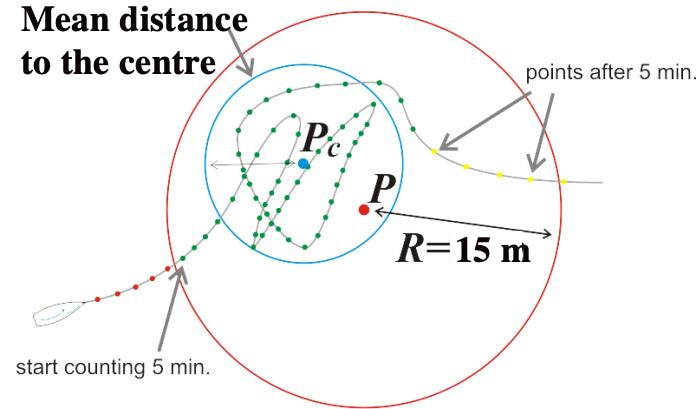
\includegraphics[width=0.6\textwidth]{station-keeping}
    \caption{Scoring procedure for the station keeping challenge}
    \label{fig:stationkeeping}
  \end{figure}

The station keeping challenge uses a single waypoint P
(see Figure \ref{fig:stationkeeping}). After entering a circle with radius $R=20m$ around the waypoint, the 
sailing vessel aims to stay as close as possible to the waypoint for 5 minutes.
The challenge is started by releasing the sailing boat at least 40m away
from the waypoint P.

\subsubsection{Scoring}
The score is calculated from the positions recorded by a tracker during the 5
minutes after first recording a position within the 20 m radius around P as
follows:
A second point $P_c$ is calculated as the average of the coordinates of all
positions. To be qualified for scoring, the point $P_c$ must be
inside the 20 m circle, regardless of the individual positions.
A circle is fitted around $P_c$, containing 95\% of the positions.
The radius of this circle around $P_c$ is $R_{min}$, and this radius is used for
scoring. The score is normalised to the vessel length overall (LOA) as 
$\frac{R_{min}}{LOA}$. 
A 5\% reduction of the score can be received for each of the individual
measurement goals, if the result is within a 20\% margin around 
the estimates by the race committee. In total three reductions of 5\%
each can be achieved. Boats are then ranked by minimum score.
%Figure 3 illustrates this procedure. The sailboat track is considered during 5
%minutes after
%entering the red circle (20m radius, centered in the reference waypoint P); the
%average of the
%coordinates of all recorded track points during the 5 mins (green dots) gives
%point Pc; the score
%is calculated with the radius of the blue circle centered in Pc that contains
%95\% of the valid
%track points. 

\subsubsection{Minimum objective}
To be scored in this contest, the vessel must enter the $R=20m$ circle around P
and continue to sail autonomously for five minutes after entering. The resulting 
point $P_c$ must be inside the 20m circle around P.

\subsection{Area scanning}
In recent years, an increasing number of attempts is made at using maritime
vessels in collaboration. A typical
collaborative task is efficiently scanning a large area.
The collaborative area scanning challenge asks teams to take the abilities and
scanning goals of other teams into consideration to optimise their own points.

The scanning task is performed over a large area around the competition, that is
structured in a grid. The boxes of the grid are assigned coordinates. Not all of
the scan area may be suitable for all boats, and it is courtesy of the teams to
choose scan goals suitable for their vessel. The
challenge runs over an extended time period over which teams can launch and
recover their vessels repeatedly either by requesting a safety boat (based on
availability; first come first serve) or by remote controlling the boat from the
pontoon to a start buoy. If a team wants to recover the boat, they must first
register the current time with the race committee, so any positions after this
time can be discarded.
During the area scanning challenge, the tracker position is made available 
to all teams live via the tracking website. Teams may update 
highlevel goals (e.g. waypoints) on their vessel remotely or change the software
on the vessel before launching again after a recovery.
Directly controlling the
actuators (e.g. remote control) is not allowed. The race committee may ask to
inspect the code determining updates to the vessel and can apply penalties if
the goal updates are used too excessively.
The boundaries of the scan area, the grid size, and the challenge start- and end time
are announced on the morning of the challenge day.
A bonus can be obtained by providing depth measurements.

The depth measurements
must be provided as one value per box, in CSV format giving a latitude and
longitude value inside the box,
the depth estimate and a timestamp for the estimate (the
timestamp is needed for tide compensation). The timestamp may be in one of the
three formats that is given in table \ref{tab:dataformats}. 
If multiple values are given, the first value in the CSV table is used.

The tracking data of all vessels is available live via the tracking website.

The area scanning challenge starts at the start time, and ends at the end
time given by the race committee on the day. The race committee may split the
challenge into two groups by randomly selecting boats for each group.

\subsubsection{Scoring}

A box in the grid is considered visited by a vessel if at least one track point
of the vessel is registered within that box within the scan time.
One point is available for each box, the final value of the box is this point 
divided by the number of vessels that visited the box. 
Each team receives the final value of all of the boxes that were visited by the
team. If a team can provide a depth estimate for a box that is within 20\% of
the race committee reference, a 5\% bonus is added to 
the final value of the box.

Boats will be ranked by the final score they achieved from boxes visited by
their vessel.

\subsubsection{Minimum objective}
To be qualified in this challenge, a vessel must register at least one track
point within the scan area during the scan time.

\subsection{Collision avoidance}
When operating in a crowded environment, autonomous sailing vessels must be able
to operate within a limited area, but also be able to avoid unexpected
obstacles. The collision avoidance challenge will evaluate the ability of a 
sailing boat to remain in a predefined channel, detect an unexpected obstacle, 
deviate from its path for obstacle avoidance and then return to its path again.
 The course area will be set with four waypoints forming a rectangle with the 
 longest side facing windward (see figure \ref{fig:obstacleavoidance}). 
Sailboats must enter the rectangle by one of the short sides, keep
sailing within the
rectangle to the opposite short side, turning back after crossing each short
side. After
completing at least two legs, a physical obstacle will be placed in the course
area before the
sailboat turns back into its direction.


  \begin{figure}[H]
    \centering
    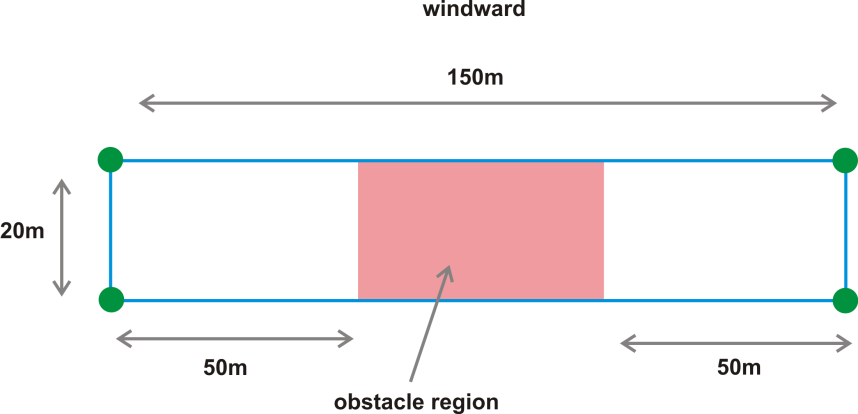
\includegraphics[width=0.8\textwidth]{obstacle-avoidance}
    \caption{Course for the obstacle avoidance challenge}
    \label{fig:obstacleavoidance}
  \end{figure}

The obstacle will occupy a large portion of the course width and will be placed
somewhere between 50m from each short side (the pink region in figure 8). 
The sailboat should log the first detection of the obstacle, deviate from its
original path without touching the obstacle, and return to the course as soon 
as possible to complete at least one more full leg. 
The “obstacle” will be made from orange balloons, transported by a motorised
vessel. The motorised vessel will do its best to stay far from the course,
keeping the obstacle on the side of the vessel that is pointing away from the
competing sailing vessel. After being placed in
position, the motorised vessel will do its best to maintain the obstacle in place.

\subsubsection{Scoring}

The runs are counted relative to the leg that has the obstacle added. Table
\ref{tab:obstacleActions} lists all actions that can be achieved during the
obstacle avoidance challenge, the leg during which they can be achieved, and
what actions are required to be successfully completed before.
Each successfully completed action is worth 1 point each. The different legs are
differentiated based on the time of crossing the short end at the start of each leg.
Where possible, successful actions are determined based on the tracking logs;
the log of action C may be provided by the team to the race committee in the
preferred format of the team. For actions D and E the race committee considers 
feedback from the safety boat
and the vessel that places the obstacle.
The teams are ranked by the number of actions achieved, the higher the number
the better. If multiple teams score a full set of actions, the time spent outside of the
rectangle during the obstacle avoidance is taken into consideration, the less
time spent outside of the rectangle, the better. The time is determined from the
timestamp of the last log position inside the rectangle to the first log position 
back within the rectangle.

\begin{table}
\centering
\begin{tabular}{l|l|p{8cm}|r}
point & leg & description & requirement \\
\hline
\hline
A & -2 & complete the entire leg within the rectangle & - \\
\hline
B & -1 & complete the entire leg within the rectangle & - \\
\hline
C & 0  & log the vessel position and time of the first detection of the obstacle & - \\
\hline
D & 0 & show visible signs of deviating from the original path & C \\
\hline
E & 0 & no collision with the obstacle & C, D\\
\hline
F & 0 & return within the square before completion of the leg & C, D, E\\
\hline
G & 1 & complete the entire leg within the rectangle & - \\
\hline
\end{tabular}
\caption{Scored actions during the obstacle avoidance challenge.}
\label{tab:obstacleActions}
\end{table}


\subsubsection{Minimum objective}
To be scored in this challenge, a vessel must enter the rectangle and complete
at least one leg within the rectangle, or it must log the detection of an
obstacle in the correct leg.
\end{document}

